\documentclass[crop,convert,tikz]{standalone}
\usetikzlibrary{datavisualization}
\begin{document}
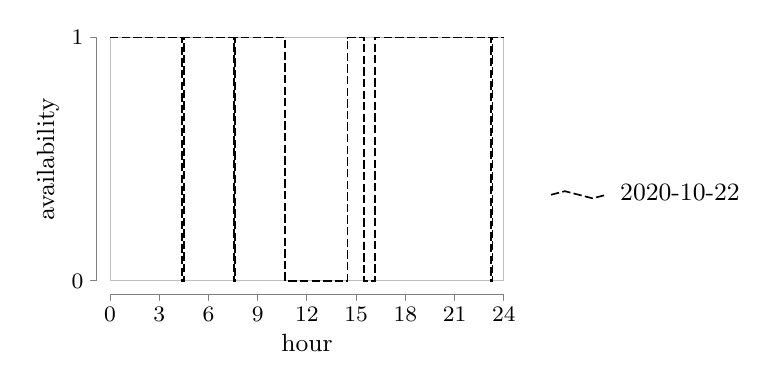
\begin{tikzpicture}
  \datavisualization[
    visualize as line/.list={a,b},
    legend={up then right},
    style sheet=vary dashing,
    scientific axes=clean,
    b={label in legend={text=2020-10-22}},
    x axis={
      label={hour},
      ticks={step=3},
    },
    y axis={
      ticks={major={at={0,1}}},
      label={availability},
    },
  ]
  data [set=b] {
    x, y
    0, 1
    4.40, 1
    4.40, 0
    4.49, 0
    4.49, 1
    7.54, 1
    7.54, 0
    7.63, 0
    7.63, 1
    10.67, 1
    10.67, 0
    14.47, 0
    14.47, 1
    15.48, 1
    15.48, 0
    16.13, 0
    16.13, 1
    23.22, 1
    23.22, 0
    23.32, 0
    23.32, 1
    24, 1
  };
\end{tikzpicture}
\end{document}
